\chapter{Bài 12. Chuyển động ném}
\begin{center}
	\textit{(3 tiết)}
\end{center}
\section{MỤC TIÊU DẠY HỌC}
\begin{center}
	\begin{longtable}{|M{2.5cm}|L{12.5cm}|M{2cm}|}
		\hline
		\thead{Biểu hiện\\ năng lực} & \thead{Mục tiêu} & \thead{STT}\\
		\hline
		\multicolumn{3}{|c|}{\textbf{ Năng lực vật lí}}\\
		\hline
		1.2 & Phân tích được các lực thành phần trong chuyển động ném. & 1\\
		\hline
		1.2 & Viết được phương trình chuyển động của vật chuyển động ném ngang. & 2\\
		\hline
		3.1 & Mô tả và giải thích được chuyển động khi vật có vận tốc không đổi theo một phương và có gia tốc không đổi theo phương vuông góc với phương này. & 3\\
		\hline
		2.4 & Thực hiện được dự án hay đề tài nghiên cứu tìm điều kiện ném vật trong không khí ở độ cao nào đó để đạt độ cao hoặc tầm xa lớn nhất. & 4\\
		\hline
		\multicolumn{3}{|c|}{\textbf{Năng lực chung}}\\
		\hline
		TC - TH& Tích cực thực hiện các nhiệm vụ đặt ra cho các nhóm.	&5 \\
		\hline
		GQVĐ - ST& Thảo luận và nêu được ý tưởng, phương án để thực hiện dự án nghiên cứu điều kiện ném vật trong không khí ở độ cao xác định để vật đạt được tầm xa lớn nhất.	&6 \\
		\hline
	\end{longtable}
\end{center}
\section{THIẾT BỊ DẠY HỌC VÀ HỌC LIỆU}
\begin{itemize}
	\item Tivi/máy chiếu;
	\item SGK.
\end{itemize}
\section{TIẾN TRÌNH DẠY HỌC}
\begin{center}
	\begin{longtable}{|L{2.75cm}|C{1.25cm}|L{5cm}|L{3.5cm}|L{4cm}|}
		\hline
		\thead{Tiến trình} & \thead{Mục\\tiêu} & \thead{Nội dung dạy học \\trọng tâm} & \thead{PP,\\ KTDH} & \thead{Phương pháp \\đánh giá}\\
		\hline
		\textbf{Hoạt động 1:} Mô tả chuyển động ném ngang&1, 5  & Mô tả chuyển động của vật ném ngang & PPDH: Đàm thoại  & GV đánh giá dựa trên câu trả lời của HS.\newline
		PP đánh giá: quan sát, nghe.  \\
		\hline
		\textbf{Hoạt động 2:} Giải thích chuyển động ném ngang&2, 3, 5  & Giải thích chuyển động của vật ném ngang & PPDH: Đàm thoại\newline KTDH: Chia sẻ cặp đôi  & GV đánh giá dựa trên câu trả lời của HS.\newline
		PP đánh giá: quan sát, nghe.  \\
		\hline
		\textbf{Hoạt động 3:} Thực hiện dự án nghiên cứu chuyển động của vật bị ném&4, 6  & Dự án nghiên cứu điều kiện ném vật trong không khí ở độ cao xác định để vật đạt được tầm xa lớn nhất & PPDH: Dạy học dự án  & GV báo cáo dự án học tập của HS.\newline
		PP đánh giá: quan sát, nghe.  \\
		\hline
		\textbf{Hoạt động 4:} Luyện tập	& 1, 2, 3 & Luyện tập bài tập chuyển động ném ngang. & PPDH:  Đàm thoại& GV đánh giá dựa trên bài tập cá nhân của học sinh.\newline
		PP đánh giá: quan sát, nghe. \\
		\hline
	\end{longtable}
\end{center}
\subsection{CÁC HOẠT ĐỘNG HỌC}
% ==========================================================================================
\hoatdong
{Mô tả chuyển động của vật ném ngang.
}
{HS mô tả được chuyển động của vật ném ngang.
}
{Câu trả lời của HS về quỹ đạo và trạng thái chuyển động của vật ném ngang (trên phương nằm ngang và phương thẳng đứng).
}
{\textit{\underline{* GV chuyển giao nhiệm vụ học tập}}
	\begin{itemize}[label=-]
		\item GV chiếu video người ném tạ cho HS xem và yêu cầu HS mô tả quỹ đạo chuyển động của vật ném ngang.\\
		\url{https://www.youtube.com/shorts/oaunkzzoFfs}
		\item GV mô tả thí nghiệm khảo sát chuyển động ném ngang trong SGK CTST trang 50 và chiếu ảnh chụp hoạt nghiệm tại nhiều thời điểm khác nhau khi thả viên bi xanh rơi tự do và viên bi đỏ theo phương ngang.
		\begin{center}
			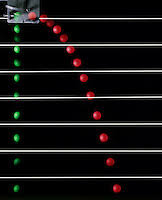
\includegraphics[scale=0.8]{figs/G10-BAI12-1}
		\end{center}
		\item GV yêu cầu HS nhận xét về trạng thái chuyển động của hai viên bi.
		\item GV nhận xét, chuẩn hóa kiến thức.
		\begin{center}
			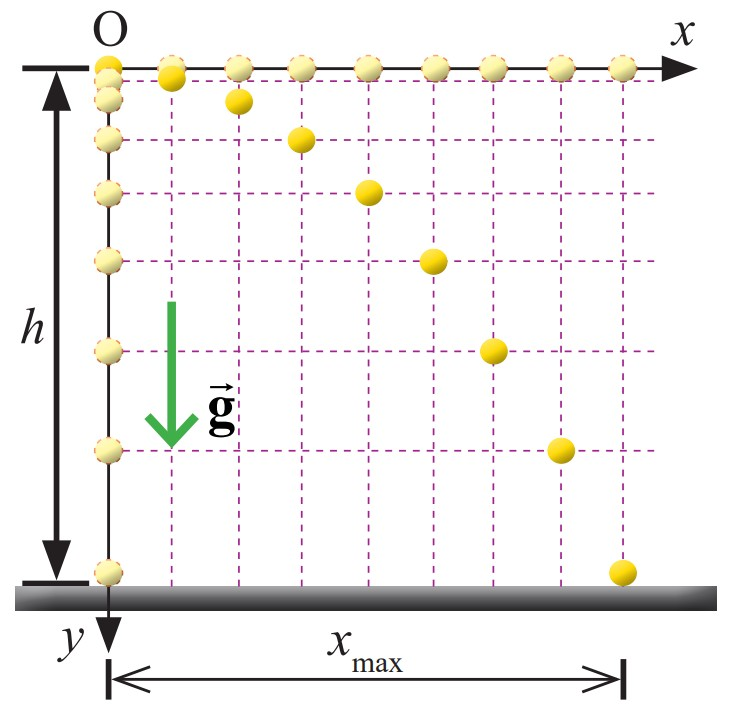
\includegraphics[scale=0.6]{figs/G10-BAI12-2}
		\end{center}
		Để đơn giản hóa quá trình khảo sát, chuyển dộng ném ngang được phân tích thành hai thành phần vuông góc với nhau trên trục $Ox$ nằm ngang và trục $Oy$ thẳng đứng. Quan sát các vị trí liên tiếp của viên bi và hình chiếu của các vị trí này trên hai trục $Ox$ và $Oy$ ta thấy:
		\begin{itemize}
			\item Quỹ đạo của viên bi có dạng đường cong.
			\item Trên trục $Ox$: hình chiếu vị trí của viên bi vàng di chuyển được những quãng đường như nhau sau những khoảng thời gian bằng nhau. Do đó trên phương này, viên bi chuyển động thẳng đều.
			\item Trên trục $Oy$: hình chiếu vị trí của viên bi đỏ hoàn toàn trùng với vị trí của viên bi xanh. Do đó trên phương này, viên bi đỏ chuyển động nhanh dần đều.
		\end{itemize}
	\end{itemize}
	\textit{\underline{* HS thực hiện nhiệm vụ học tập}}\\
HS chú ý lắng nghe và trả lời câu hỏi của GV.\\
	\textit{\underline{* HS báo cáo kết quả nhiệm vụ học tập}}
	\begin{itemize}[label=-]
		\item GV lần lượt mời HS trả lời câu hỏi.
		\item Các HS khác theo dõi và nhận xét.
		\item GV chỉnh lí và hợp thức hóa kiến thức.
	\end{itemize}
}
% ==========================================================================================
\hoatdong
{Giải thích chuyển động của vật ném ngang.
}
{HS vận dụng kiến thức phần động học và động lực học để xây dựng phương trình chuyển động của vật ném ngang.
}
{Phương trình chuyển động của vật ném ngang.
}
{\textit{\underline{* GV chuyển giao nhiệm vụ học tập}}
	\begin{itemize}[label=-]
		\item GV yêu cầu HS thảo luận nhóm đôi và xác định các lực tác dụng lên viên bi trong quá trình chuyển động (bỏ qua lực cản của không khí).
		\item GV yêu cầu HS xác định gia tốc, từ đó suy ra trạng thái chuyển động của vật ném ngang trên các trục $Ox$ và $Oy$.
	\end{itemize}
	\begin{center}
		\begin{tikzpicture}[scale=1, transform shape]  %horizontal projection
			%variable definitions
			\def\g{-9.8} %gravity
			\def\v{10} %velocity
			\def\ang{51} %angle
			\def\s{0.125}
			\pgfmathsetmacro{\c}{{(-1*(2/\g)*\v*sin(\ang))/2}}
			\pgfmathsetmacro{\a}{{(-1*(2/\g)*\v*sin(\ang))*.9}}
			
			\begin{axis}[
				width=.6\linewidth, %set bigger width
				height=3in,
				xmin={{\v*cos(\ang)*\c}},xmax=10, %{\v*cos(\ang)*\a+\s*\v*cos(\ang)}
				ymin=0,ymax={\v*\c*sin(\ang)+0.5*\g*(\c^2)},
				axis x line = top,
				every axis y label/.style={at={(axis description cs:0,-0.05)}},
				every axis x label/.style={at={(axis description cs:1.05,1)},anchor=west},
				xlabel=$x$,
				ylabel=$y$,
				axis y line = left,
				y axis line style={<-},
				x axis line style={<->},
				ticks = none,clip=false,
				]
				
				\tikzset{every mark/.append style={fill=red}}
				
				%flight path
				\addplot[
				dashed,
				domain={\v*cos(\ang)*\c}:10,
				samples=100,]
				{{\g*(x^2)/(2*\v^2*cos(\ang)^2)+x*tan(\ang)}};
				
				%vector at end
				\pgfmathsetmacro{\a}{{(-1*(2/\g)*\v*sin(\ang))*.9}}
				\coordinate (E) at (axis cs:{\v*cos(\ang)*\a},{\v*\a*sin(\ang)+0.5*\g*(\a^2)}){};
				\coordinate (F) at (axis cs:{\v*cos(\ang)*\a+\s*\v*cos(\ang))}, {\v*\a*sin(\ang)+0.5*\g*\a^2+\s*(\v*sin(\ang)+\g*\a)});
				\draw[thick,->](E)--(F);
				%			node[midway,sloped,above]{$\vec{V}$};
				\draw[densely dashed,thick,->](E)--(F |- E);
				%			node[midway,above]{$\vec{V}_x$};
				\draw[densely dashed,thick,->](E)--(F-| E);
				%			node[midway,left]{$\vec{V}_y$};
				
				\path plot[mark=*] coordinates {(E)};
				
				%vector at start
				\pgfmathsetmacro{\c}{{(-1*(2/\g)*\v*sin(\ang))/2}}
				\coordinate (L) at (axis cs:{\v*cos(\ang)*\c},{\v*\c*sin(\ang)+0.5*\g*(\c^2)});
				\coordinate (M) at (axis cs:{\v*cos(\ang)*\c+\s*\v*cos(\ang))},{\v*\c*sin(\ang)+0.5*\g*\c^2+\s*(\v*sin(\ang)+\g*\c)});
				\draw[thick,->](L)--(M)
				node[near end,sloped,above]{$\vec{v}_0$};
				
				\path plot[mark=*] coordinates {(L)};
				
				%vector 1/2 down
				\pgfmathsetmacro{\d}{{(-1*(2/\g)*\v*sin(\ang))*0.6}}
				\coordinate (P) at (axis cs:{\v*cos(\ang)*\d},{\v*\d*sin(\ang)+0.5*\g*(\d^2)});
				\coordinate (Q) at (axis cs:{(\v*cos(\ang)*\d+\s*\v*cos(\ang))},{\v*\d*sin(\ang)+0.5*\g*\d^2+\s*(\v*sin(\ang)+\g*\d)});
				\draw[thick,->](P)--(Q)
				%node[midway,sloped,above]{$\vec{V}$}
				;
				\draw[densely dashed,thick,->](P)--(Q|-P);
				%			node[midway,above]{$\vec{V}_x$};
				\draw[densely dashed,thick,->](P)--(Q-|P);
				%			node[midway,left]{$\vec{V}_y$};
				
				\path plot[mark=*] coordinates {(P)};
				
				%vector 3/4 down
				\pgfmathsetmacro{\f}{{(-1*(2/\g)*\v*sin(\ang))*0.7}}
				\coordinate (R) at (axis cs:{\v*cos(\ang)*\f},{\v*\f*sin(\ang)+0.5*\g*(\f^2)});
				\coordinate (S) at (axis cs:{(\v*cos(\ang)*\f+\s*\v*cos(\ang))},{\v*\f*sin(\ang)+0.5*\g*\f^2+\s*(\v*sin(\ang)+\g*\f)});
				\draw[thick,->](R)--(S);
				%			node[near end,above]{$\vec{v}$};
				\draw[densely dashed,thick,->](R)--(S|-R);
				%			node[near end,above,]{$\vec{v}_x$};
				\draw[densely dashed,thick,->](R)--(S-|R);
				%			node[near end,left]{$\vec{v}_y$};
				
				\path plot[mark=*] coordinates {(R)};
				
				%vector 1/4 down
				\pgfmathsetmacro{\e}{{(-1*(2/\g)*\v*sin(\ang))*0.8}}
				\coordinate (T) at (axis cs:{\v*cos(\ang)*\e},{\v*\e*sin(\ang)+0.5*\g*(\e^2)});
				\coordinate (U) at (axis cs:{(\v*cos(\ang)*\e+\s*\v*cos(\ang))},{\v*\e*sin(\ang)+0.5*\g*\e^2+\s*(\v*sin(\ang)+\g*\e)});
				\draw[thick,->,blue](T)--(U)
				node[near end,right=2mm]{$\vec{v}$};
				\draw[densely dashed,thick,->,blue](T)--(U|-T)
				node[near end,above]{$\vec{v}_x$};
				\draw[densely dashed,thick,->,blue](T)--(U-|T)
				node[near end,left]{$\vec{v}_y$};
				
				\path plot[mark=*] coordinates {(T)};
			\end{axis}
		\end{tikzpicture}
		\captionof{figure}{Phân tích chuyển động ném ngang.}
	\end{center}
	\item GV yêu cầu HS từ trạng thái chuyển động của vật đã phân tích ở trên kết hợp các công thức động học đã học, hãy xác định phương trình vận tốc và phương trình tọa độ của vật trên các phương $Ox$ và $Oy$.\\
	\textit{\underline{* HS thực hiện nhiệm vụ học tập}}
	\begin{itemize}[label=-]
		\item HS chú ý lắng nghe hướng dẫn của GV.
		\item HS thảo luận nhóm đôi để thực hiện các nhiệm vụ học tập GV chuyển giao.
	\end{itemize}
	\textit{\underline{* HS báo cáo kết quả nhiệm vụ học tập}}
	\begin{itemize}[label=-]
		\item GV mời đại diện 2 nhóm HS lên trình bày kết quả thảo luận (1 HS viết phương trình chuyển động trên trục $Ox$ và 1 HS viết phương trình chuyển động trên trục $Oy$).
		\item Các HS khác theo dõi và nhận xét.
		\item GV nhận xét và chuẩn hóa kiến thức.
	\end{itemize}
}
% ==========================================================================================
\hoatdong
{Thực hiện dự án nghiên cứu chuyển động của vật bị ném.
}
{HS thực hiện được dự án hay đề tài nghiên cứu tìm điều kiện ném vật trong không khí ở độ cao nào đó để đạt độ cao hoặc tầm xa lớn nhất.
}
{\begin{itemize}
		\item Các nhóm quay video các thí nghiệm đã thực hiện, quay báo cáo.
		\item Nộp lại bản báo cáo đã làm cho giáo viên cùng video.
	\end{itemize}
}
{\textit{\underline{* GV chuyển giao nhiệm vụ học tập}}
	\begin{itemize}[label=-]
		\item GV chia lớp thành 6 nhóm để thực hiện dự án.
		\item GV giới thiệu dự án cho HS với các yêu cầu như sau:
		\begin{itemize}
			\item \textbf{Chuẩn bị:}
			\begin{itemize}
				\item Dụng cụ có thể dùng để bắn các viên bi nhỏ với những lực có độ lớn khác nhau, theo các phương khác nhau.
				\item Thước đo độ dài, thước đo góc.
				\item Địa điểm làm thí nghiệm có các độ cao khác nhau, đảm bảo an toàn tuyệt đối khi tiến hành thí nghiệm.
			\end{itemize}
			\item \textbf{Tiến hành:}
			\begin{itemize}
				\item Báo cáo ngắn gọn về lý thuyết : Để ném ngang một vật đạt tầm bay xa lớn nhất thì phải chọn độ cao như thế nào? Để ném xiên một vật đạt tầm bay xa lớn nhất thì phải chọn góc ném thế nào?
				\item Báo cáo phương án làm thí nghiệm để kiểm tra dự đoán, thực hiện thí nghiệm, rút ra kết luận.
			\end{itemize}
		\end{itemize}
		\item GV giao cho học sinh thực hiện ngoài giờ học trên lớp và nộp báo cáo để trao đổi, chia sẻ và đánh giá vào các thời điểm phù hợp trong kế hoạch giáo dục môn học/hoạt động giáo dục của giáo viên.
	\end{itemize}
	\textit{\underline{* HS thực hiện nhiệm vụ học tập}}\\
	HS thực hiện dự án học tập theo nhóm được phân công.\\
	\textit{\underline{* HS báo cáo kết quả nhiệm vụ học tập}}\\
	HS nộp video và bản báo cáo dự án cho GV.
}
\hoatdong{
	Luyện tập.
}
{
	HS sử dụng các phương trình chuyển động ném ngang để giải bài tập.
}
{
	Bài tập cá nhân của học sinh.
}
{
	\textit{\underline{* GV chuyển giao nhiệm vụ học tập}}\\
	GV lần lượt chuyển giao từng bài tập, yêu cầu HS hoạt động cá nhân để giải.\\
	\textit{\underline{* HS thực hiện nhiệm vụ học tập}}\\
	HS \textit{(làm việc cá nhân)}:  Giải bài tập trong phiếu bài tập được GV giao. 
	
	GV: Theo dõi để phát hiện các HS gặp khó khăn, từ đó đưa ra sự định hướng, hỗ trợ phù hợp cho mỗi HS.\\
	\textit{\underline{* HS báo cáo kết quả thực hiện nhiệm vụ học tập}}\\
	GV: Mời HS lên bảng giải bài tập.
	
	HS: Đặt câu hỏi, góp ý.
	
	GV: Chỉnh lí, hợp thức hoá kiến thức.
}
\section{HỒ SƠ DẠY HỌC}
\subsection{NỘI DUNG DẠY HỌC}
\begin{enumerate}[label=\bfseries\Roman*.]
	\item \textbf{Mô tả chuyển động ném ngang}\\
	Xét chuyển động ném ngang (trong mặt phẳng như hình) với vận tốc ban đầu $\vec{v}_0$, vật luôn có gia tốc bằng gia tốc rơi tự do $\vec{g}$ thẳng đứng hướng xuống.
	\begin{center}
		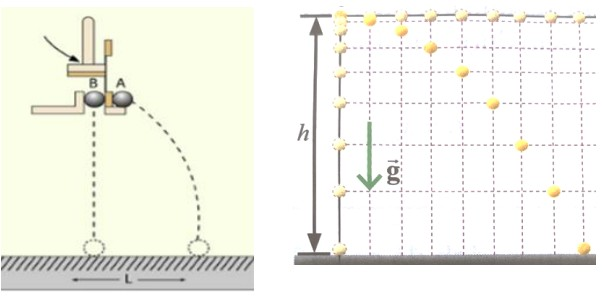
\includegraphics[scale=0.7]{figs/G10-BAI12-3}
	\end{center}
	\textit{Hình chiếu chuyển động của vật lên phương nằm ngang là chuyển động thẳng đều, lên phương thẳng đứng là chuyển động rơi tự do.}
	\item \textbf{Giải thích chuyển động ném ngang}\\
	\begin{enumerate}[label=\bfseries \alph*.]
		\item \textbf{Chọn hệ quy chiếu:} Chọn hệ trục tọa độ $Oxy$ như hình và gốc thời gian lúc ném vật.
			\begin{center}
			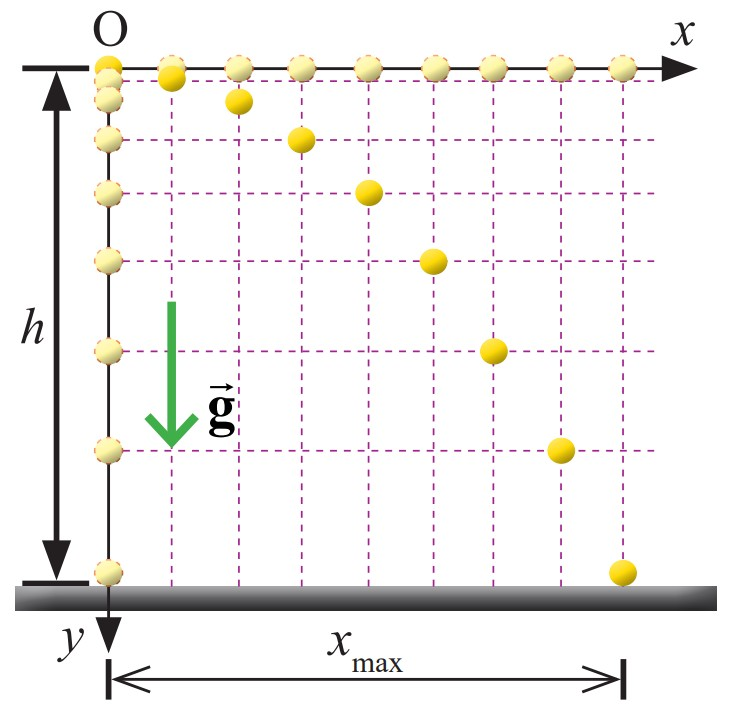
\includegraphics[scale=0.6]{figs/G10-BAI12-2}
		\end{center}
		\begin{itemize}
			\item \textbf{Trên trục $Ox$:}
			\begin{itemize}
				\item Gia tốc: $a_x=0$, vật chuyển động thẳng đều trên $Ox$.
				\item Vận tốc: $v_x=v_0$ là hằng số.
				\item Phương trình chuyển động thẳng đều: $x=v_0t$.
			\end{itemize}
			\item \textbf{Trên trục $Oy$:}
			\begin{itemize}
				\item Gia tốc: $a_y=g$
				\item Vận tốc: $v_y=gt$
				\item Phương trình chuyển động: $y=\dfrac{1}{2}gt^2$.
			\end{itemize}
		\end{itemize}
		\item \textbf{Phương trình quỹ đạo, thời gian rơi, tầm bay xa, vận tốc của vật ở thời điểm $t$}
		\begin{itemize}
			\item Phương trình quỹ đạo: $y=\dfrac{g}{2v^2}x^2$.\\
			\textit{Vậy quỹ đạo chuyển động của vật là một nhánh của đường parabol}.
			\item Thời gian rơi: $t=\sqrt{\dfrac{2h}{g}}$.
			\item Tầm xa: $L=x_{\max}=v_0t=v_0\sqrt{\dfrac{2h}{g}}$.\\
			\textit{($L$ là khoảng cách từ hình chiếu của điểm ném trên mặt đất đến điểm rơi.)}
			\item Vận tốc của vật ở thời điểm $t$: $\vec{v}=\vec{v}_x+\vec{v}_y$ mà $\vec{v}_x\bot\vec{v}_{y}\Rightarrow v=\sqrt{v^2_x+v^2_y}$ với $v_x=v_0$, $v_y=gt$.
		\end{itemize}
	\end{enumerate}
\end{enumerate}
\subsection{BÀI TẬP}
\textbf{* BÀI TẬP TRẮC NGHIỆM}
\setcounter{ex}{0}
% ===================================================================
\begin{ex}
	Một vật rơi có khối lượng $m$, được ném ngang với vận tốc ban đầu $v_0$ ở độ cao $h$. Bỏ qua sức cản của không khí. Thời gian rơi	
	\choice
	{chỉ phụ thuộc vào $m$}
	{\True chỉ phụ thuộc vào $h$}
	{phụ thuộc $v_0$ và $h$}
	{phụ thuộc vào $m$, $v_0$, $h$}
	\loigiai{}
\end{ex}
% ===================================================================
\begin{ex}
	Một vật có khối lượng $m$, được ném ngang với vận tốc ban đầu $v_0$ ở độ cao $h$. Bỏ qua sức cản của không khí. Tầm bay xa của vật phụ thuộc vào
	\choice
	{$m$ và $v_0$}
	{$m$ và $h$}
	{$v_0$ và $h$}
	{$m$, $v_0$ và $h$}
	\loigiai{}
\end{ex}
% ===================================================================
\begin{ex}
	Quỹ đạo chuyển động của vật ném ngang là một 
	\choice
	{đường thẳng}
	{đường tròn}
	{đường xoắn ốc}
	{nhánh parabol}
	\loigiai{}
\end{ex}
% ===================================================================
\begin{ex}
	Quả cầu I có khối lượng  gấp đôi quả cầu II. Cùng một lúc tại độ cao $h$, quả cầu I được thả rơi còn quả cầu II được ném theo phương ngang. Bỏ qua sức cản của không khí. Chọn phát biểu đúng?
	\choice
	{Quả cầu I chạm đất trước}
	{Quả cầu II chạm đất trước}
	{Cả hai quả cầu I và II chạm đất cùng một lúc}
	{Chưa đủ cơ sở để kết luận}
	\loigiai{}
\end{ex}
% ===================================================================
\begin{ex}
	Từ trên một máy bay đang chuyển động đều theo phương ngang người ta thả một vật rơi xuống đất. Bỏ qua sức cản không khí. Nhận xét nào sau đây là \textbf{sai}?	
	\choice
	{Người quan sát đứng trên mặt đất nhìn thấy quỹ đạo của vật là một phần của parabol}
	{Người quan sát đứng trên máy bay nhìn thấy quỹ đạo của vật là một phần của parabol}
	{Người quan sát đứng trên máy bay nhìn thấy quỹ đạo của vật là một đường thẳng đứng}
	{Vị trí chạm đất ở ngay dưới máy bay theo phương thẳng đứng}
	\loigiai{}
\end{ex}
% ===================================================================
\begin{ex}
	Trong chuyển động ném ngang, gia tốc của vật tại một vị trí bất kì luôn có đặc điểm là hướng theo
	\choice
	{phương ngang, cùng chiều chuyển động}
	{phương ngang, ngược chiều chuyển động}
	{phương thẳng đứng, chiều từ dưới lên trên}
	{phương thẳng đứng, chiều từ trên xuống dưới}
	\loigiai{}
\end{ex}
% ===================================================================
\begin{ex}
	Một vật ở độ cao $h$ được ném theo phương ngang với tốc độ $v_0=\SI{50}{\meter/\second}$ và rơi chạm đất sau $\SI{10}{\second}$. Lấy $g=\SI{10}{\meter/\second^2}$. Tầm xa của vật là	
	\choice
	{$\SI{400}{\meter}$}
	{$\SI{200}{\meter}$}
	{$\SI{300}{\meter}$}
	{$\SI{500}{\meter}$}
	\loigiai{}
\end{ex}
% ===================================================================
\begin{ex}
	Ném một vật nhỏ theo phương nằm ngang với tốc độ ban đầu là $\SI{5}{\meter/\second}$, tầm xa của vật là $\SI{15}{\meter}$. Thời gian rơi của vật là
	\choice
	{$\SI{2}{\second}$}
	{$\SI{4}{\second}$}
	{$\SI{1}{\second}$}
	{$\SI{3}{\second}$}
	\loigiai{}
\end{ex}
% ===================================================================
\begin{ex}
	Một vật ở độ cao $h$ được ném theo phương ngang với tốc độ $v_0$ và rơi chạm đất sau $\SI{5}{\second}$. Lấy $g=\SI{10}{\meter/\second^2}$. Vật được ném từ độ cao nào
	\choice
	{\SI{100}{\meter}}
	{\SI{125}{\meter}}
	{\SI{200}{\meter}}
	{\SI{30}{\meter}}
	\loigiai{}
\end{ex}
% ===================================================================
\begin{ex}
	Một quả bóng được ném theo phương ngang với tốc độ ban đầu $v_0=\SI{20}{\meter/\second}$ và rơi xuống đất sau $\SI{3}{\second}$. Lấy $g=\SI{10}{\meter/\second^2}$. Bỏ qua sức cản không khí. Quả bóng được ném từ độ cao
	\choice
	{\SI{45}{\meter}}
	{\SI{30}{\meter}}
	{\SI{60}{\meter}}
	{\SI{90}{\meter}}
	\loigiai{}
\end{ex}
% ===================================================================
\begin{ex}
	Một viên đạn được bắn theo phương ngang từ một khẩu súng đặt ở độ cao $\SI{20}{\meter}$ so với mặt đất. Tốc độ của đạn lúc vừa ra khỏi nòng súng là $\SI{300}{\meter/\second}$. Lấy $g=\SI{10}{\meter/\second^2}$. Điểm đạn rơi xuống cách điểm bắn theo phương ngang là
	\choice
	{\SI{600}{\meter}}
	{\SI{360}{\meter}}
	{\SI{480}{\meter}}
	{\SI{180}{\meter}}
	\loigiai{}
\end{ex}
% ===================================================================
\begin{ex}
	Phương trình quỹ đạo của một vật được ném theo phương ngang có dạng $y=x^2/10$. Lấy $g=\SI{9.8}{\meter/\second^2}$. Tốc độ ban đầu của vật là 
	\choice
	{\SI{7}{\meter/\second}}
	{\SI{5}{\meter/\second}}
	{\SI{2.5}{\meter/\second}}
	{\SI{4.9}{\meter/\second}}
	\loigiai{}
\end{ex}
% ===================================================================
\begin{ex}
	Một vật được ném theo phương ngang với tốc độ $v_0=\SI{15}{\meter/\second}$ và rơi chạm đất sau $\SI{2}{\second}$. Lấy $g=\SI{10}{\meter/\second^2}$. Khi chạm đất vật đạt tốc độ
	\choice
	{\SI{25}{\meter/\second}}
	{\SI{15}{\meter/\second}}
	{\SI{20}{\meter/\second}}
	{\SI{35}{\meter/\second}}
	\loigiai{}
\end{ex}
% ===================================================================
\begin{ex}
	Một vật được ném ngang với tốc độ $v_0=\SI{30}{\meter/\second}$, ở độ cao $h=\SI{80}{\meter}$. Lấy $g=\SI{10}{\meter/\second^2}$. Tầm bay xa và tốc độ của vật khi chạm đất là	
	\choice
	{\SI{120}{\meter}; \SI{50}{\meter/\second}}
	{\SI{50}{\meter}; \SI{120}{\meter/\second}}
	{\SI{120}{\meter}; \SI{70}{\meter/\second}}
	{\SI{70}{\meter}; \SI{120}{\meter/\second}}
	\loigiai{}
\end{ex}
% ===================================================================
\begin{ex}
	Một vật được ném theo phương ngang với tốc độ ban đầu $v_0=\SI{8}{\meter/\second}$. Lấy $g=\SI{10}{\meter/\second^2}$. Sau khi ném $\SI{2}{\second}$, phương của vận tốc và phương ngang hợp nhau một góc 	
	\choice
	{\SI{37.5}{\degree}}
	{\SI{84.7}{\degree}}
	{\SI{62.8}{\degree}}
	{\SI{68.2}{\degree}}
	\loigiai{}
\end{ex}
\textbf{* BÀI TẬP TỰ LUẬN}
\setcounter{ex}{0}
% ======================================================================
\begin{ex}
	Từ độ cao $\SI{45}{\meter}$ so với mặt đất, một vật được ném theo phương ngang với vận tốc đầu $v_0$. Khi chạm đất, vector vận tốc của vật hợp với phương ngang góc $\SI{30}{\degree}$. Tìm $v_0$ và tầm xa vật đạt được. Lấy $g=\SI{9.8}{\meter/\second^2}$.
	\loigiai{$v_0=\xsi{30\sqrt{3}}{\meter/\second}$; $L=\SI{156}{\meter}$.} 
\end{ex}
% ======================================================================
\begin{ex}
	Một người trượt tuyết rời khỏi đường trượt theo phương ngang với vận tốc $\SI{25}{\meter/\second}$. Người này đáp xuống một dốc nghiêng $\SI{35}{\degree}$ so với phương ngang ở vị trí cách điểm xuất phát bao xa? Lấy $g=\SI{9.8}{\meter/\second^2}$.
	\loigiai{$d=\SI{109}{\meter}$}
\end{ex}
% ======================================================================
\begin{ex}
	Một quả cầu được ném theo phương ngang từ độ cao $\SI{80}{\meter}$. Sau khi chuyển động được $\SI{3}{\second}$ vận tốc quả cầu hợp với phương ngang góc $\SI{45}{\degree}$. Lấy $g=\SI{10}{\meter/\second^2}$.
	\begin{enumerate}[label=\alph*)]
		\item Tìm tốc độ ban đầu của quả cầu.
		\item Qủa cầu sẽ chạm đất lúc nào? Ở đâu? Với tốc độ bao nhiêu?
	\end{enumerate}	
	\loigiai{
		\begin{enumerate}[label=\alph*)]
			\item $v_0=\SI{30}{\meter/\second}$.
			\item $t=\SI{4}{\second}$; $L=\SI{120}{\meter}$; $v=\SI{50}{\meter/\second}$.
		\end{enumerate}
	}
\end{ex}

% ======================================================================
\begin{ex}
	\immini{Một kiến trúc sư cảnh quan đang lên kế hoạch xây dựng một thác nước nhân tạo trong công viên thành phố. Một kênh dẫn nằm ngang ở độ cao $h=\SI{2.35}{\meter}$ dẫn nước với tốc độ $\SI{1.70}{\meter/\second}$ chảy vào một bể chứa bên dưới như hình vẽ. Lấy $g=\SI{9.8}{\meter/\second^2}$.
		\begin{enumerate}[label=\alph*)]
			\item Tính tầm xa của nước khi đổ xuống bể chứa.
			\item Để bán kế hoạch của mình cho hội đồng thành phố, kiến trúc sư muốn xây dựng một mô hình theo tỷ lệ tiêu chuẩn, có kích thước bằng 1 phần 12 kích thước thật. Nước trong kênh trong mô hình phải chảy với tốc độ bao nhiêu?
	\end{enumerate}	}
	{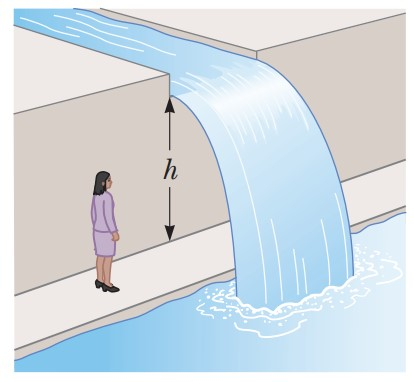
\includegraphics[scale=0.7]{../figs/G10-BTNEMNGANG2}}
	
	\loigiai{}
\end{ex}
% ======================================================================
\begin{ex}
	\immini{Một chiếc xe tải chở đầy dưa hấu dừng lại đột ngột để tránh lao xuống sông do cây cầu đã bị cuốn trôi. Việc dừng xe đột ngột khiến một số quả dưa văng khỏi xe tải. Một quả dưa rời khỏi mui xe tải với tốc độ ban đầu $v_i=\SI{10}{\meter/\second}$ theo phương ngang. Mặt cắt ngang của bờ sông có dạng nửa parabol $y^2=16x$, với đỉnh là vị trí ban đầu của quả dưa hấu và $x,y$ đều đo bằng mét. Quả dưa hấu va vào bờ sông ở tọa độ bằng bao nhiêu?	Lấy $g=\SI{9.8}{\meter/\second^2}$.}
	{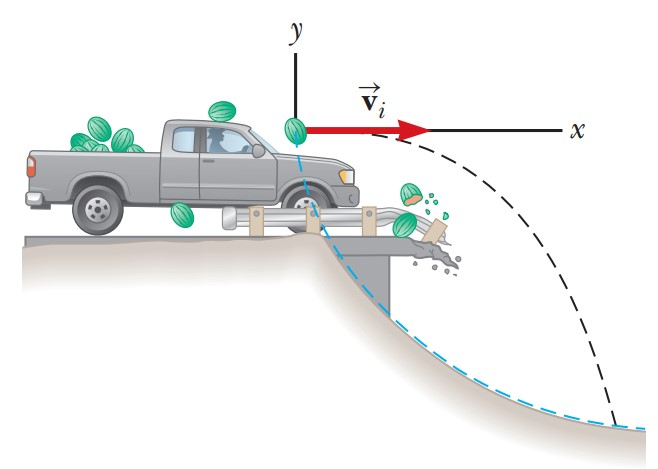
\includegraphics[scale=0.6]{../figs/G10-BTNEMNGANG2-2}}
	\loigiai{}
\end{ex}
% ======================================================================
\begin{ex}
	\immini{Trong hình bên, bốn lá sen nhô lên khỏi mặt nước và một con ếch đang ở ngồi trên bờ hồ. Cho rằng độ cao của bờ hồ và lá sen so với mặt nước lần lượt là $H=6h$, $h_a=h_b=4h$, $h_c=h_d=h$. Ếch và tâm của hai lá sen a, b cùng nằm trên một mặt phẳng thẳng đứng. Giao điểm của thân bốn lá sen với mặt nước là bốn đỉnh của một hình vuông song song với bờ sông và có chiều dài cạnh bằng $\ell$. Khoảng cách theo phương ngang giữa lá sen a và bờ hồ cũng là $\ell$. Xem con ếch chuyển động như vật ném ngang với gia tốc trọng trường $g$.}
	{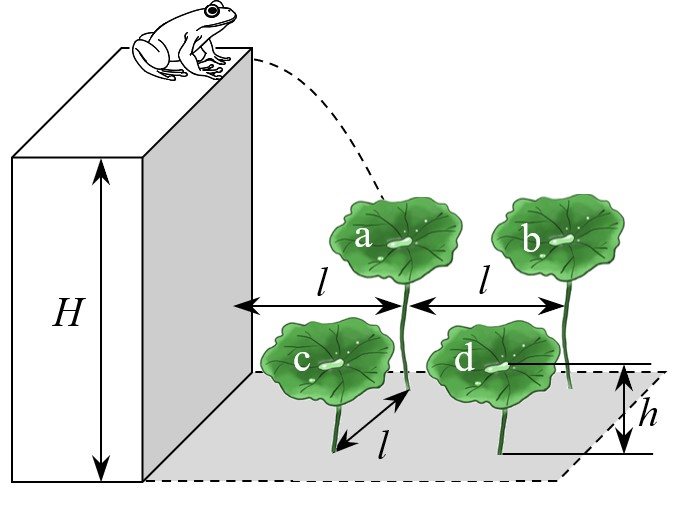
\includegraphics[scale=0.6]{../figs/G10-BTNEMNGANG2-5}}
	\begin{enumerate}[label=\alph*)]
		\item Sau một cú nhảy, con ếch đã đậu thành công trên lá sen a. Tìm tốc độ ban đầu của con ếch.
		\item Tốc độ nhảy ban đầu của con ếch ứng với sự rơi trên lá sen nào là nhỏ nhất? Giải thích một cách tường minh.
	\end{enumerate}
	\loigiai{}
\end{ex}
% ======================================================================
\begin{ex}
	\immini{Chó sói Wile E. Coyote cố gắng một lần nữa để bắt chú gà lôi thông minh Road Runner. Sói Wile E. mang một đôi giày trượt patin trợ lực mới để tạo ra gia tốc không đổi $\SI{15}{\meter/\second^2}$ trên phương ngang như hình bên. Con sói xuất phát từ trạng thái nghỉ cách mép vách đá $\SI{70}{\meter}$ vào thời điểm gà lôi vượt qua nó và lao về hướng vách đá. Lấy $g=\SI{9.8}{\meter/\second^2}$.
		\begin{enumerate}[label=\alph*)]
			\item Nếu gà lôi chạy với tốc độ không đổi, hãy tìm tốc độ tối thiểu của nó để đến được vách đá trước khi con sói bắt kịp.
			\item Nếu vách đá cao $\SI{100}{\meter}$ so với chân núi, hãy tìm nơi con sói rơi xuống. \textit{(Giả sử giày trượt của Wile E. vẫn còn hoạt động khi nó đang bay và thành phần phần gia tốc theo phương ngang anh ta vẫn bằng $\SI{15}{\meter/\second^2}$ không đổi).}
	\end{enumerate}}
	{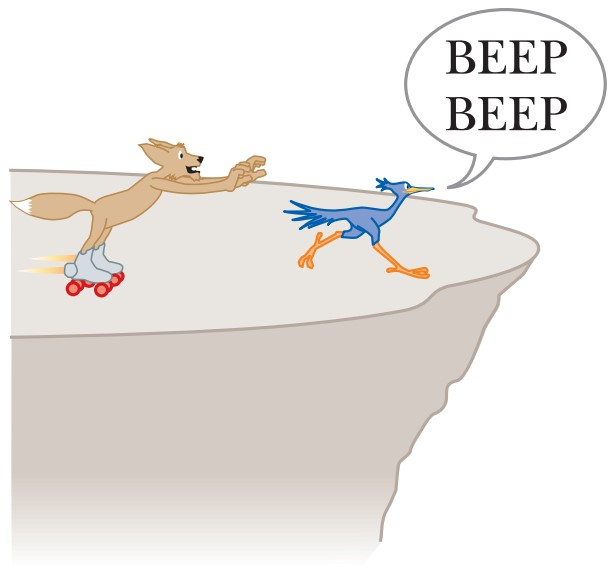
\includegraphics[scale=0.6]{../figs/G10-BTNEMNGANG2-4}}
	
	\loigiai{}
\end{ex}
% ======================================================================
\begin{ex}
	\immini{Một máy bay ném bom, bay theo phương ngang ở độ cao $H=\SI{500}{\meter}$ so với mặt đất, chuyển động nhanh dần đều với gia tốc $a=\SI{2}{\meter/\second^2}$ và các quả bom được thả sau những khoảng thời gian bằng nhau $t=\SI{0.5}{\second}$. Tìm khoảng cách giữa các điểm rơi của quả bom thứ 9 và thứ 11 trên mặt đất nếu quả bom thứ nhất được thả ra khi vận tốc của máy bay là $v_0=\SI{100}{\meter/\second}$. Cho $g=\SI{10}{\meter/\second^2}$ và bỏ qua sức cản của không khí.}
	{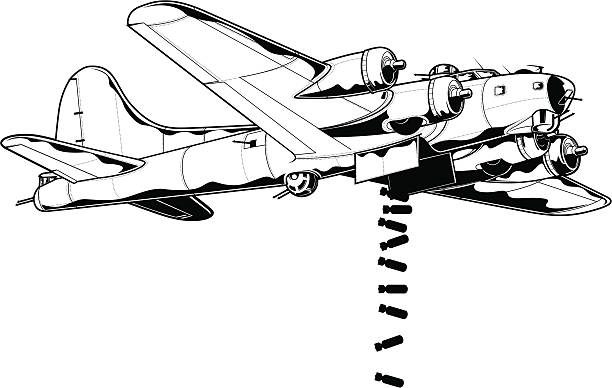
\includegraphics[scale=0.7]{../figs/G10-BTNEMNGANG2-3}}
	\loigiai{$\Delta s=L+s_{11}-s_9=\SI{129}{\meter}$.}
\end{ex}